\documentclass{article} \usepackage{graphicx} \usepackage[utf8]{inputenc} \usepackage{polski} \author{C and bash} \title{Równiania} \begin{document} 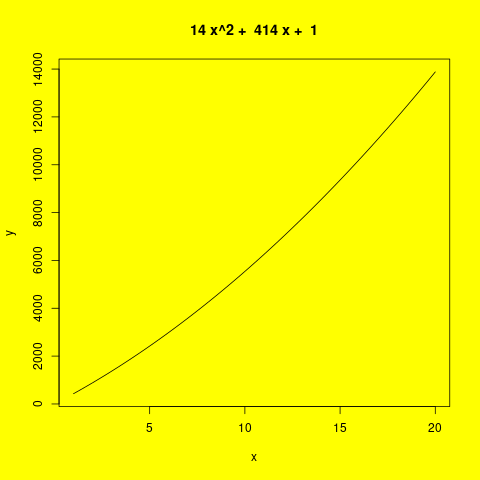
\includegraphics{output.png} \maketitle
Mamy funkcje 1.0x^2 + 7.0x + 5.0 \Delta = 7.0^2 - 4\times1.0\times5.0 Niema pierwiastkow \begin{tabular}{|c|c|} \hline 20.0 & 545.0 \ \hline 21.0 & 593.0 \ \hline 22.0 & 643.0 \ \hline 23.0 & 695.0 \ \hline 24.0 & 749.0 \ \hline 25.0 & 805.0 \ \hline \end{tabular}
\\\
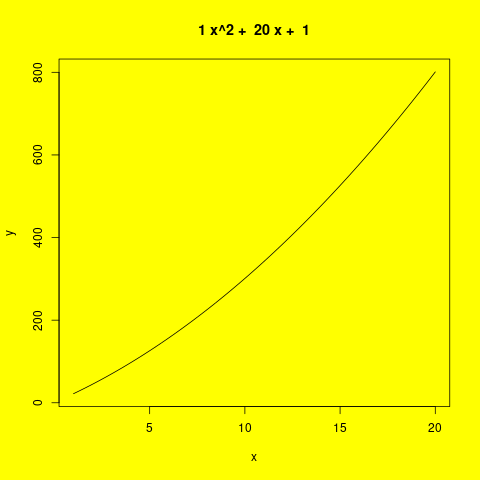
\includegraphics[width=0.5\textwidth]{res/0img.png}
\newline 7311051 nanoseconds elpased
\clearpage 
Mamy funkcje 10.0x^2 + 13.0x + 11.0 \Delta = 13.0^2 - 4\times10.0\times11.0 Niema pierwiastkow \begin{tabular}{|c|c|} \hline 20.0 & 4271.0 \ \hline 20.0 & 4271.0 \ \hline 20.0 & 4271.0 \ \hline 20.0 & 4271.0 \ \hline 20.0 & 4271.0 \ \hline 20.0 & 4271.0 \ \hline 20.0 & 4271.0 \ \hline 20.0 & 4271.0 \ \hline 20.0 & 4271.0 \ \hline 20.0 & 4271.0 \ \hline 20.0 & 4271.0 \ \hline 20.0 & 4271.0 \ \hline 20.0 & 4271.0 \ \hline 20.0 & 4271.0 \ \hline 20.0 & 4271.0 \ \hline 20.0 & 4271.0 \ \hline 20.0 & 4271.0 \ \hline 20.0 & 4271.0 \ \hline \end{tabular}
\\\
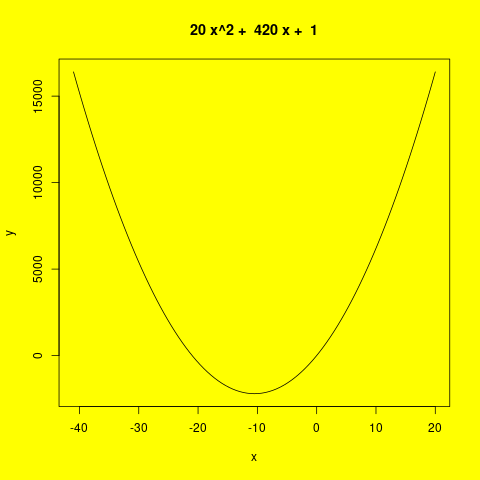
\includegraphics[width=0.5\textwidth]{res/1img.png}
\newline 6140198 nanoseconds elpased
\clearpage 
Mamy funkcje 16.0x^2 + 10.0x + 9.0 \Delta = 10.0^2 - 4\times16.0\times9.0 Niema pierwiastkow \begin{tabular}{|c|c|} \hline 9.0 & 1395.0 \ \hline 10.0 & 1709.0 \ \hline 11.0 & 2055.0 \ \hline 12.0 & 2433.0 \ \hline \end{tabular}
\\\
\includegraphics[width=0.5\textwidth]{res/2img.png}
\newline 4481434 nanoseconds elpased
\clearpage 
Mamy funkcje 6.0x^2 + 3.0x + 11.0 \Delta = 3.0^2 - 4\times6.0\times11.0 Niema pierwiastkow \begin{tabular}{|c|c|} \hline 17.0 & 1796.0 \ \hline 17.0 & 1796.0 \ \hline 17.0 & 1796.0 \ \hline 17.0 & 1796.0 \ \hline 17.0 & 1796.0 \ \hline 17.0 & 1796.0 \ \hline 17.0 & 1796.0 \ \hline 17.0 & 1796.0 \ \hline 17.0 & 1796.0 \ \hline 17.0 & 1796.0 \ \hline 17.0 & 1796.0 \ \hline \end{tabular}
\\\
\includegraphics[width=0.5\textwidth]{res/3img.png}
\newline 5581863 nanoseconds elpased
\clearpage 
Mamy funkcje 16.0x^2 + 1.0x + 7.0 \Delta = 1.0^2 - 4\times16.0\times7.0 Niema pierwiastkow \begin{tabular}{|c|c|} \hline 1.0 & 24.0 \ \hline \end{tabular}
\\\
\includegraphics[width=0.5\textwidth]{res/4img.png}
\newline 4238027 nanoseconds elpased
\clearpage 
Mamy funkcje 19.0x^2 + 12.0x + 3.0 \Delta = 12.0^2 - 4\times19.0\times3.0 Niema pierwiastkow \begin{tabular}{|c|c|} \hline 6.0 & 759.0 \ \hline 8.0 & 1315.0 \ \hline 10.0 & 2023.0 \ \hline 12.0 & 2883.0 \ \hline 14.0 & 3895.0 \ \hline 16.0 & 5059.0 \ \hline 18.0 & 6375.0 \ \hline 20.0 & 7843.0 \ \hline 22.0 & 9463.0 \ \hline 24.0 & 11235.0 \ \hline 26.0 & 13159.0 \ \hline \end{tabular}
\\\
\includegraphics[width=0.5\textwidth]{res/5img.png}
\newline 4337134 nanoseconds elpased
\clearpage 
Mamy funkcje 9.0x^2 + 18.0x + 13.0 \Delta = 18.0^2 - 4\times9.0\times13.0 Niema pierwiastkow \begin{tabular}{|c|c|} \hline 9.0 & 904.0 \ \hline 11.0 & 1300.0 \ \hline 13.0 & 1768.0 \ \hline 15.0 & 2308.0 \ \hline 17.0 & 2920.0 \ \hline 19.0 & 3604.0 \ \hline 21.0 & 4360.0 \ \hline 23.0 & 5188.0 \ \hline 25.0 & 6088.0 \ \hline 27.0 & 7060.0 \ \hline 29.0 & 8104.0 \ \hline \end{tabular}
\\\
\includegraphics[width=0.5\textwidth]{res/6img.png}
\newline 4272708 nanoseconds elpased
\clearpage 
Mamy funkcje 16.0x^2 + 4.0x + 10.0 \Delta = 4.0^2 - 4\times16.0\times10.0 Niema pierwiastkow \begin{tabular}{|c|c|} \hline 4.0 & 282.0 \ \hline 4.0 & 282.0 \ \hline 4.0 & 282.0 \ \hline 4.0 & 282.0 \ \hline 4.0 & 282.0 \ \hline 4.0 & 282.0 \ \hline 4.0 & 282.0 \ \hline 4.0 & 282.0 \ \hline 4.0 & 282.0 \ \hline 4.0 & 282.0 \ \hline 4.0 & 282.0 \ \hline 4.0 & 282.0 \ \hline 4.0 & 282.0 \ \hline 4.0 & 282.0 \ \hline 4.0 & 282.0 \ \hline 4.0 & 282.0 \ \hline 4.0 & 282.0 \ \hline \end{tabular}
\\\
\includegraphics[width=0.5\textwidth]{res/7img.png}
\newline 5403608 nanoseconds elpased
\clearpage 
Mamy funkcje 17.0x^2 + 16.0x + 14.0 \Delta = 16.0^2 - 4\times17.0\times14.0 Niema pierwiastkow \begin{tabular}{|c|c|} \hline 11.0 & 2247.0 \ \hline 11.0 & 2247.0 \ \hline 11.0 & 2247.0 \ \hline 11.0 & 2247.0 \ \hline 11.0 & 2247.0 \ \hline 11.0 & 2247.0 \ \hline 11.0 & 2247.0 \ \hline \end{tabular}
\\\
\includegraphics[width=0.5\textwidth]{res/8img.png}
\newline 4516179 nanoseconds elpased
\clearpage 
Mamy funkcje 13.0x^2 + 5.0x + 19.0 \Delta = 5.0^2 - 4\times13.0\times19.0 Niema pierwiastkow \begin{tabular}{|c|c|} \hline 9.0 & 1117.0 \ \hline 9.0 & 1117.0 \ \hline 9.0 & 1117.0 \ \hline 9.0 & 1117.0 \ \hline \end{tabular}
\\\
\includegraphics[width=0.5\textwidth]{res/9img.png}
\newline 4234326 nanoseconds elpased
\clearpage 
Mamy funkcje 3.0x^2 + 19.0x + 12.0 \Delta = 19.0^2 - 4\times3.0\times12.0 Niema pierwiastkow \begin{tabular}{|c|c|} \hline 15.0 & 972.0 \ \hline 16.0 & 1084.0 \ \hline 17.0 & 1202.0 \ \hline 18.0 & 1326.0 \ \hline 19.0 & 1456.0 \ \hline 20.0 & 1592.0 \ \hline 21.0 & 1734.0 \ \hline 22.0 & 1882.0 \ \hline 23.0 & 2036.0 \ \hline 24.0 & 2196.0 \ \hline 25.0 & 2362.0 \ \hline 26.0 & 2534.0 \ \hline 27.0 & 2712.0 \ \hline 28.0 & 2896.0 \ \hline 29.0 & 3086.0 \ \hline 30.0 & 3282.0 \ \hline \end{tabular}
\\\
\includegraphics[width=0.5\textwidth]{res/10img.png}
\newline 4025708 nanoseconds elpased
\clearpage 
\newline 4025708 nanoseconds elpased for entire script
\end{document}
